\documentclass{article}
\usepackage{graphicx}
\usepackage{amsmath}
\usepackage{enumitem}
\usepackage{float}

\graphicspath{{images/}}


\author{Janati Imrane, Leroy Tanguy, Ouarghi Yanis, Sadiki Ilias}
\date{}   

\begin{document}

\title{Gesture recognition system}
\maketitle

\section{Introduction}
As part of the Machine Learning course, 
we developed a gesture recognition system based on 3D data. 
The project consisted in classifying digits (from 0 to 9) 
drawn in the air by different users using supervised classification techniques. 
After a phase of data exploration and preprocessing, 
we implemented a baseline method (Dynamic Time Warping) 
as well as a more advanced model, to compare their performances 
in both user-dependent and user-independent settings. 
This report presents our approach, the methodological choices made, 
as well as the results obtained.

\section{Exploratory data analysis}
Nous disposons de 1 000 fichiers représentant les chiffres de 0 à 9, écrits par 10 individus différents, chacun ayant répété chaque chiffre 10 fois. Cela correspond à un total de 85 095 coordonnées à traiter.
( Une étude exploratoire est essentielle pour mieux comprendre la structure et les caractéristiques de ces données, et ainsi orienter efficacement les étapes de modélisation. )
Un premier aspect important à analyser est la longueur des séquences, c’est-à-dire le nombre de points ou coordonnées enregistrés par fichier. Cette information est cruciale, notamment pour les modèles basés sur le deep learning, qui requièrent souvent que toutes les séquences d’entrée aient une taille identique.
Nos observations révèlent une forte variabilité dans le nombre de points par séquence. Par exemple, le chiffre 7 est souvent représenté par moins de points que les autres chiffres, ce qui complique l’uniformisation des séquences et, par conséquent, l’apprentissage automatique. 
Cette variabilité est corrélée avec la durée de réalisation du geste, bien que nous n’ayons pas intégré cette dernière dans nos analyses .

\begin{figure}[H]
    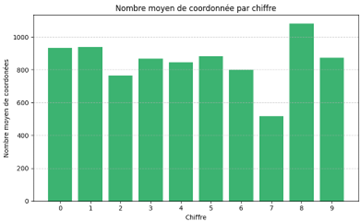
\includegraphics[width=\textwidth]{coord_par_chiffres.png}
\end{figure}

Nous avons également examiné la variabilité des gestes entre utilisateurs. Les résultats montrent que l’utilisateur 10 a tendance à écrire certains chiffres différemment par rapport aux autres, particulièrement sur les premiers chiffres. Aucun chiffre ne ressort comme particulièrement difficile à interpréter globalement, à l’exception potentielle du chiffre “0”, qui présente une plus grande variabilité.
Pour illustrer, voici la projection en 3D d’un “0” réalisé par l’utilisateur 10, montrant une forme atypique comparée aux autres utilisateurs.

\begin{figure}[H]
    \centering
    \begin{minipage}{0.64\textwidth}
        \centering
        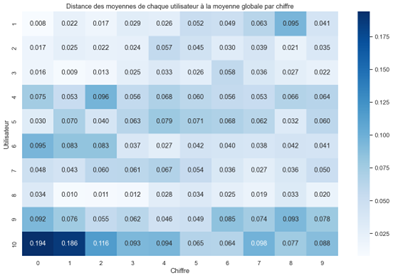
\includegraphics[width=\textwidth]{dist_moyennes_user_moyenne_globale.png}
    \end{minipage}
    \hfill
    \begin{minipage}{0.35\textwidth}
        \centering
        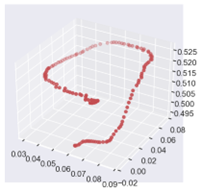
\includegraphics[width=\textwidth]{chiffre_moche.png}
    \end{minipage}
\end{figure}

\section{Preprocessing}
Pour garantir la qualité et la robustesse des modèles, nous avons procédé à une normalisation des données. Cette standardisation a été réalisée en tenant compte des groupes, des itérations, et des utilisateurs, afin d’atténuer l’impact des valeurs extrêmes et du bruit. Cette étape facilite la détection de gestes atypiques, tels que le “0” de l’utilisateur 10.
Nous avons ensuite construit deux jeux de données distincts :

\begin{itemize}
    \item Données brutes normalisées : Contenant l’ensemble des informations originales standardisées. Ces données sont destinées à un modèle basé sur des mesures de distance non supervisées.
    \item Données avec séquences de longueur fixe : Pour permettre l’utilisation de modèles plus complexes, nécessitant des entrées de taille constante, nous avons appliqué un resampling. Ce processus inclut :
    \item Une interpolation linéaire pour générer des points supplémentaires quand une séquence est trop courte.
    \item Un sous-échantillonnage uniforme pour réduire le nombre de points dans les séquences trop longues, en conservant la forme générale du geste.
\end{itemize}
Cette uniformisation est une étape indispensable pour assurer la cohérence des données en entrée, améliorer la stabilité de l’entraînement et la performance des modèles.

\section{Models}

\subsection{DTW + KNN}
Notre premier modèle combine deux méthodes : le Dynamic Time Warping (DTW) et le k-Nearest Neighbors (k-NN).
Le DTW est une technique qui permet de mesurer la similarité entre des séries temporelles, même si elles ont des vitesses ou des longueurs différentes. Même si on ne se concentre pas vraiment sur la dimension temps dans notre cas, le  DTW est pratique car il ne demande pas de modifier nos données. Il peut comparer directement des séquences en 3D, ce qui correspond bien à nos coordonnées (x, y, z), et il n’impose pas que toutes les séquences aient la même longueur.
Le k-NN, quant à lui, est un algorithme de classification simple qui attribue une catégorie à un nouvel échantillon en regardant ses voisins les plus proches. Ici, on utilise la distance calculée par le DTW pour définir qui sont ces voisins. Le k-NN est facile à comprendre et à utiliser, et il fonctionne sans besoin d’entraînement compliqué ou de gros changements sur les données.
Le principal problème avec cette méthode, c’est qu’elle peut être assez lente, surtout quand on a beaucoup de données à traiter, car le calcul du DTW est coûteux en temps.
Malgré ça, la combinaison DTW + k-NN reste une bonne option pour notre projet, notamment parce qu’elle gère bien les différences de taille entre les séquences sans perdre d’informations importantes. 

\subsection{CNN}
tfou3lik
\section{Feature selection}
Dans notre deuxième approche, nous avons choisi une méthode de feature selection afin d’extraire un ensemble de caractéristiques statistiques et géométriques des gestes bruts plutôt que de les traiter directement. 
This is going to allow us to transform every sequence of points into a fixed vector of features, making the input data less complex and compatible with models of classical classification like random forest or decision trees. 
Cette méthode est relativement simple et rapide à entrainer, et permet d’obtenir de bonnes performances. Revoyons da manière un peu plus détaillée le déroulé de ce modèle et comment nous l’avons appliqué à notre problème. 
Pour chaque séquence de geste qui est représentée comme une série de points dans l’espace, nous avons extraits 75 caractéristiques numériques. Chaque geste aura ainsi un vecteur de caractéristiques d’une longueur de 75 données. 
Nous avons d’abord extrait des données statistiques classiques comme la moyenne, l’écart-type, les minima, maxima ou encore la médiane.
A tout cela va s’ajouter les 10 premiers coefficients de la transformée de Fourrier discrète. Cet outil mathématique va en effet permettre de transformer les séquences de gestes en coefficients, dont on ne gardera que les 10 les plus importants. 
Nous avons également pu calculer des variables liées à la dynamique du mouvement, en nous basant sur les différences temporelles des coordonnées. On a alors créé des variables de moyenne, d’écart-type, de maximum et de médiane sur la vitesse et l’accélération des gestes. 
Enfin, afin de capter la complexité du geste, nous avons estimé les angles entre chaque segment, un segment étant la liaison entre 2 points successifs, qui composent le geste. On a alors pu calculer la moyenne de ces angles ainsi que l’écart-type pour chaque geste. Les 2 dernières variables sélectionnées concernent la longueur totale parcourue pour le geste, ainsi que l’angle entre le vecteur global obtenu pour notre geste et l’axe des abscisses. 

A partir de ces vecteurs de caractéristiques, 
nous avons décidé d’entrainer un modèle d’Extreme Gradient Boosting (XGBoost). 
Nous étions à la base parti sur un arbre aléatoire classique, 
mais en raison d’un manque de précision dans les résultats, 
nous sommes passés à un modèle plus sophistiqué. 
En effet, le XGBoost est un algorithme plus adapté 
puisqu’il construit des arbres séquentiels 
qui corrigent les erreurs des précédents (apprentissage par renforcement). 
Il permet en plus d’avoir un meilleur contrôle de l’overfitting, 
d’être plus précis et pondère de manière plus efficace les features, 
c'est-à-dire savoir prioriser et donner de l’importance à certaines variables \cite{chen2016}. 
Here is its objective function :

\[ 
\mathcal{L}^{(t)} = \sum_{i=1}^{n} [g_i*f_{t}(x_i) + \frac{1}{2} h_i f_{t}^2(x_i)] + \gamma T + \frac{1}{2} \lambda \sum_{j=1}^{T} w_{j}^2 + \frac{1}{2} \alpha \sum_{j=1}^{T} |w_j| 
\]

\begin{tabular}{llll}
$g_i$ & gradient of the loss term & $h_i$ & hessian of the loss term \\
$f_t$ & new tree to learn         & $w_j$ & leaf score \\
$T$   & number of leaves          & $\gamma, \lambda, \alpha$ & regularization hyperparameters \\
\end{tabular}


\section{Combination}

Afin d’améliorer une dernière fois nos prédictions, 
nous avons combiné nos deux modèles les plus performants 
en termes de rapidité et de précision : le CNN et XGB. 
Après avoir analysé les forces et faiblesses de chacun, 
nous avons mis en place un système de vote conditionnel.
Chaque séquence test est évaluée une fois par chaque modèle. 
En cas de désaccord, une règle simple détermine lequel des deux doit être suivi, 
en fonction du chiffre prédit. Par exemple, nous avons observé que 
lorsque XGB prédit les chiffres 0, 2 ou 8, ses résultats sont 
généralement plus fiables que ceux du CNN, qui a tendance à mal les classer. 
Dans ces cas précis, nous choisissons donc de faire confiance à la prédiction de XGB. 
Pour les autres classes, où le CNN montre de meilleures performances globales, 
c’est sa prédiction qui est retenue.

\section{Comparison of results}

Le but de cette partie est de comparer les résultats obtenus avec les baseline methods and more state-of-art methods. Nous choisissons d’utiliser les résultats de la méthode de combination pour la partie avancée puisqu’elle celle-ci a pour but de donner de meilleurs résultats que ses deux composantes. Ensuite, il sera également nécessaire de comparer les résultats en fonction du type de data splitting qui a été utilisé. Pour ce projet, deux méthodes de splitting. Il existe deux types d’évaluation. En user-independent, on teste le modèle sur un utilisateur jamais vu. On utilise la méthode leave-one-user-out.  A chaque fois, un utilisateur est mis de côté pour le test, et le modèle est entraîné sur les 9 autres. Cela permet d’évaluer la capacité à généraliser à un nouvel utilisateur. En user-dependent, on teste sur des gestes déjà vus, mais sur des exemples différents. Pour chaque utilisateur, un exemple par geste est gardé pour le test, et les autres servent à l’entraînement. Cela mesure la capacité à reconnaître des gestes connus mais exécutés différemment \cite{bulling2014}.
Commençons par la comparaison entre les 2 méthodes de splitting. 
Comme on pouvait s’y attendre, que ça soit pour la baseline ou la méthode avancée, 
nous avons de meilleurs résultats lorsque le splitting est en user-dependent. 
En effet, pour la baseline, nous obtenons une précision de 92,7\% en user-independent contre 98,6\% en user-dependent. 
Pour la combinaison avancée, nous obtenons 96,8\% en user-independent et 98,4\% en user-dependent. 
On obtient généralement une meilleure précision en user-dependent, 
car le modèle a déjà vu des exemples très similaires à ceux du test. 
Il s'entraîne et teste sur les mêmes utilisateurs, 
donc il reconnaît plus facilement leurs façons de faire les gestes. 
En revanche, en user-independent, le modèle doit prédire les gestes d’un utilisateur totalement nouveau, 
ce qui est plus difficile car chaque personne a sa propre manière d’exécuter les gestes.
Pour la comparaison entre la méthode baseline et la méthode avancée, 
nous observons de meilleurs résultats en moyenne. 
En effet, en user-independent, la précision est de 92,7\% avec la baseline alors qu’elle est de 96,8\% pour l’autre. 
Cela répond à notre objectif qui était d’obtenir de meilleurs résultats avec les méthodes plus avancées. 
On peut notamment observer le nombre d’erreurs pour chaque geste des méthodes à travers les matrices de confusion suivantes :

\begin{figure}[h]
    \centering
    \begin{minipage}{0.4\textwidth}
        \centering
        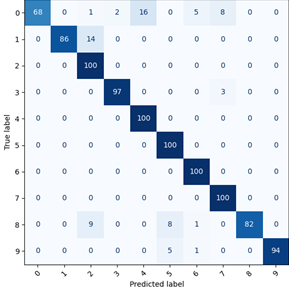
\includegraphics[width=\textwidth]{baseline_user-independent.png}
        \caption{baseline user-independent}
    \end{minipage}
    \hfill
    \begin{minipage}{0.4\textwidth}
        \centering
        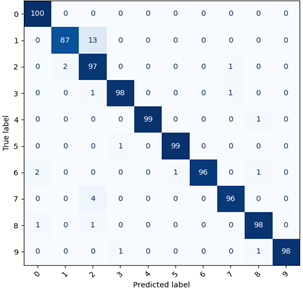
\includegraphics[width=\textwidth]{combined_user-independent.png}
        \caption{combined user-independent}
    \end{minipage}
\end{figure}

Cependant, en user-dependent, la baseline affiche des résultats très légèrement supérieurs, 
avec une précision de 98,6\% contre 98,4\% pour la combinaison avancée. 
Même si la méthode avancée (CNN + features) est plus élaborée, 
elle fait légèrement moins bien que la baseline (DTW + KNN) en user-dependent. 
C’est normal, car dans ce cas, le modèle revoit les mêmes utilisateurs entre l’entraînement et le test. 
Et comme DTW + KNN est très bon pour comparer des gestes déjà vus, il suffit largement dans ce contexte. 
La méthode avancée, elle, est surtout utile quand les conditions sont plus dures, comme en user-independent, 
où il faut s’adapter à un nouvel utilisateur (Bulling et Al., 2014).

\section{Conclusion}
Best model? user/iter out?  accuracy/overfitting?

\bibliographystyle{plain}
\bibliography{bibl}


\end{document}